\RequirePackage[final]{graphicx}
\documentclass[draft]{article}

\usepackage{amsmath,amssymb,amsfonts}
\usepackage{algorithmic}
\usepackage{slashbox}
\usepackage{float}
\usepackage[table, dvipsnames]{xcolor}
\usepackage{pifont}% http://ctan.org/pkg/pifont
\usepackage{slashbox}
\usepackage{cite}
\usepackage{bm}
\usepackage{graphicx}
\usepackage{textcomp}
\usepackage{grffile}
\usepackage[final]{pdfpages}
\usepackage{pdflscape}
\usepackage{tcolorbox}
\usepackage{pifont}
\usepackage{adjustbox}
\usepackage{bbm}

\usepackage{tikz}
\usepackage{colortbl}
\usepackage[normalem]{ulem}
\usepackage{multirow}
\usepackage{hhline}
\usepackage{nicematrix}
\usepackage{array}
\usepackage{xparse}
\usepackage{xifthen}
\usepackage[final]{listings}
\usepackage[pagebackref=true,breaklinks=true]{hyperref}
\usepackage[numbers]{natbib}
\usepackage{cleveref}
\usepackage{ifdraft}
\usepackage[inline]{enumitem}
\usepackage{makecell}

\usepackage{subcaption}
\usepackage{mwe}
%\usepackage[a4paper, total={6in, 8in}]{geometry}

\usepackage[parfill]{parskip}


\usepackage{tasks}


\usepackage[font={small,it,color = black},labelfont={normalfont, bf},tableposition=top,labelsep=period]{caption}

\hypersetup{final = true}
\hypersetup{
    colorlinks = true,
    linkcolor={red!70!black},
    citecolor={blue!70!black},
    urlcolor={blue!80!black}
}

\tcbuselibrary{most}

\ifdraft{%
    \usepackage[colorinlistoftodos]{todonotes}}{ % draft with TODOs
    \usepackage[disable]{todonotes} % final without TODOs
}

\SetLabelAlign{myright}{\hss\llap{$#1$}}
\newlist{where}{description}{1}
\setlist[where]{labelwidth=2cm,labelsep=1em,
                        leftmargin=!,align=myright,font=\normalfont}

\makeatletter
\DeclareRobustCommand{\iscircle}{\mathord{\mathpalette\is@circle\relax}}
\newcommand\is@circle[2]{%
  \begingroup
  \sbox\z@{\raisebox{\depth}{$\m@th#1\bigcirc$}}%
  \sbox\tw@{$#1\square$}%
  \resizebox{!}{\ht\tw@}{\usebox{\z@}}%
  \endgroup
}
\makeatother

\def\BibTeX{{\rm B\kern-.05em{\sc i\kern-.025em b}\kern-.08em
    T\kern-.1667em\lower.7ex\hbox{E}\kern-.125emX}}

\definecolor{Joris}{rgb}{0.19, 0.55, 0.91}
\newcommand{\Joris}[1]{\todo[color = Joris, inline]{\textbf{Joris: } #1}}

\definecolor{bananayellow}{rgb}{1.0, 0.88, 0.21}
\newcommand{\Struc}[1]{\todo[color = bananayellow, inline]{\textbf{Structuur: } #1}}

\definecolor{Jan}{rgb}{1, 0.55, 0}
\newcommand{\Jan}[1]{\todo[color = Jan, inline]{\textbf{Jan.: } #1}}

\definecolor{Etienne}{rgb}{1, 1, 0}
\newcommand{\Etienne}[1]{\todo[color = Etienne, inline]{\textbf{Etienne: } #1}}

\definecolor{Rob}{rgb}{0, 1, 0}
\newcommand{\Rob}[1]{\todo[color = Rob, inline]{\textbf{Rob: } #1}}

\definecolor{Mark}{rgb}{1, 0, 1}
\newcommand{\Mark}[1]{\todo[color = Mark, inline]{\textbf{Mark: } #1}}

\definecolor{lavendermagenta}{rgb}{0.93, 0.51, 0.93}
\newcommand{\tcjoris}[1]{\begin{tcolorbox}[colback = lavendermagenta!15, colframe = lavendermagenta, breakable = unlimited]
#1
\end{tcolorbox}
}

\definecolor{amber}{rgb}{1.0, 0.75, 0.0}
\newcommand{\NOGREF}{\todo[backgroundcolor = amber!15, bordercolor = amber, linecolor = amber]
{Nog verwijzen!}
}

\definecolor{slateblue}{rgb}{0.42, 0.35, 0.8}
\newcommand{\NOG}[1]{\todo[backgroundcolor = slateblue!15, bordercolor = slateblue, linecolor = slateblue]
{Nog zeggen: #1}
}

\definecolor{fireenginered}{rgb}{0.81, 0.09, 0.13}
\definecolor{gold(web)(golden)}{rgb}{1.0, 0.84, 0.0}
\newcommand{\TOD}[1]{\todo[backgroundcolor = fireenginered, bordercolor = gold(web)(golden), inline, textcolor = gold(web)(golden), shadow]{#1}}

\newtheorem{conjecture}{Conjecture}
\newtheorem{evidence}{Evidence}
\newtheorem{assumption}{Assumption}
\usepackage{amsthm}
\theoremstyle{definition}
\newtheorem{definition}{Definition}
%%%%%%%%%%%%% Hier komen de Wiskundige Commands

\DeclareMathOperator*{\argmax}{arg\,max}
\DeclareMathOperator*{\argmin}{arg\,min}
\newcommand{\cmark}{\ding{51}}%
\newcommand{\xmark}{\ding{55}}%





\usetikzlibrary{calc}
\usetikzlibrary{decorations.pathreplacing}
\usetikzlibrary{arrows}

\begin{document}
\resizebox*{0.95\linewidth}{!}{
    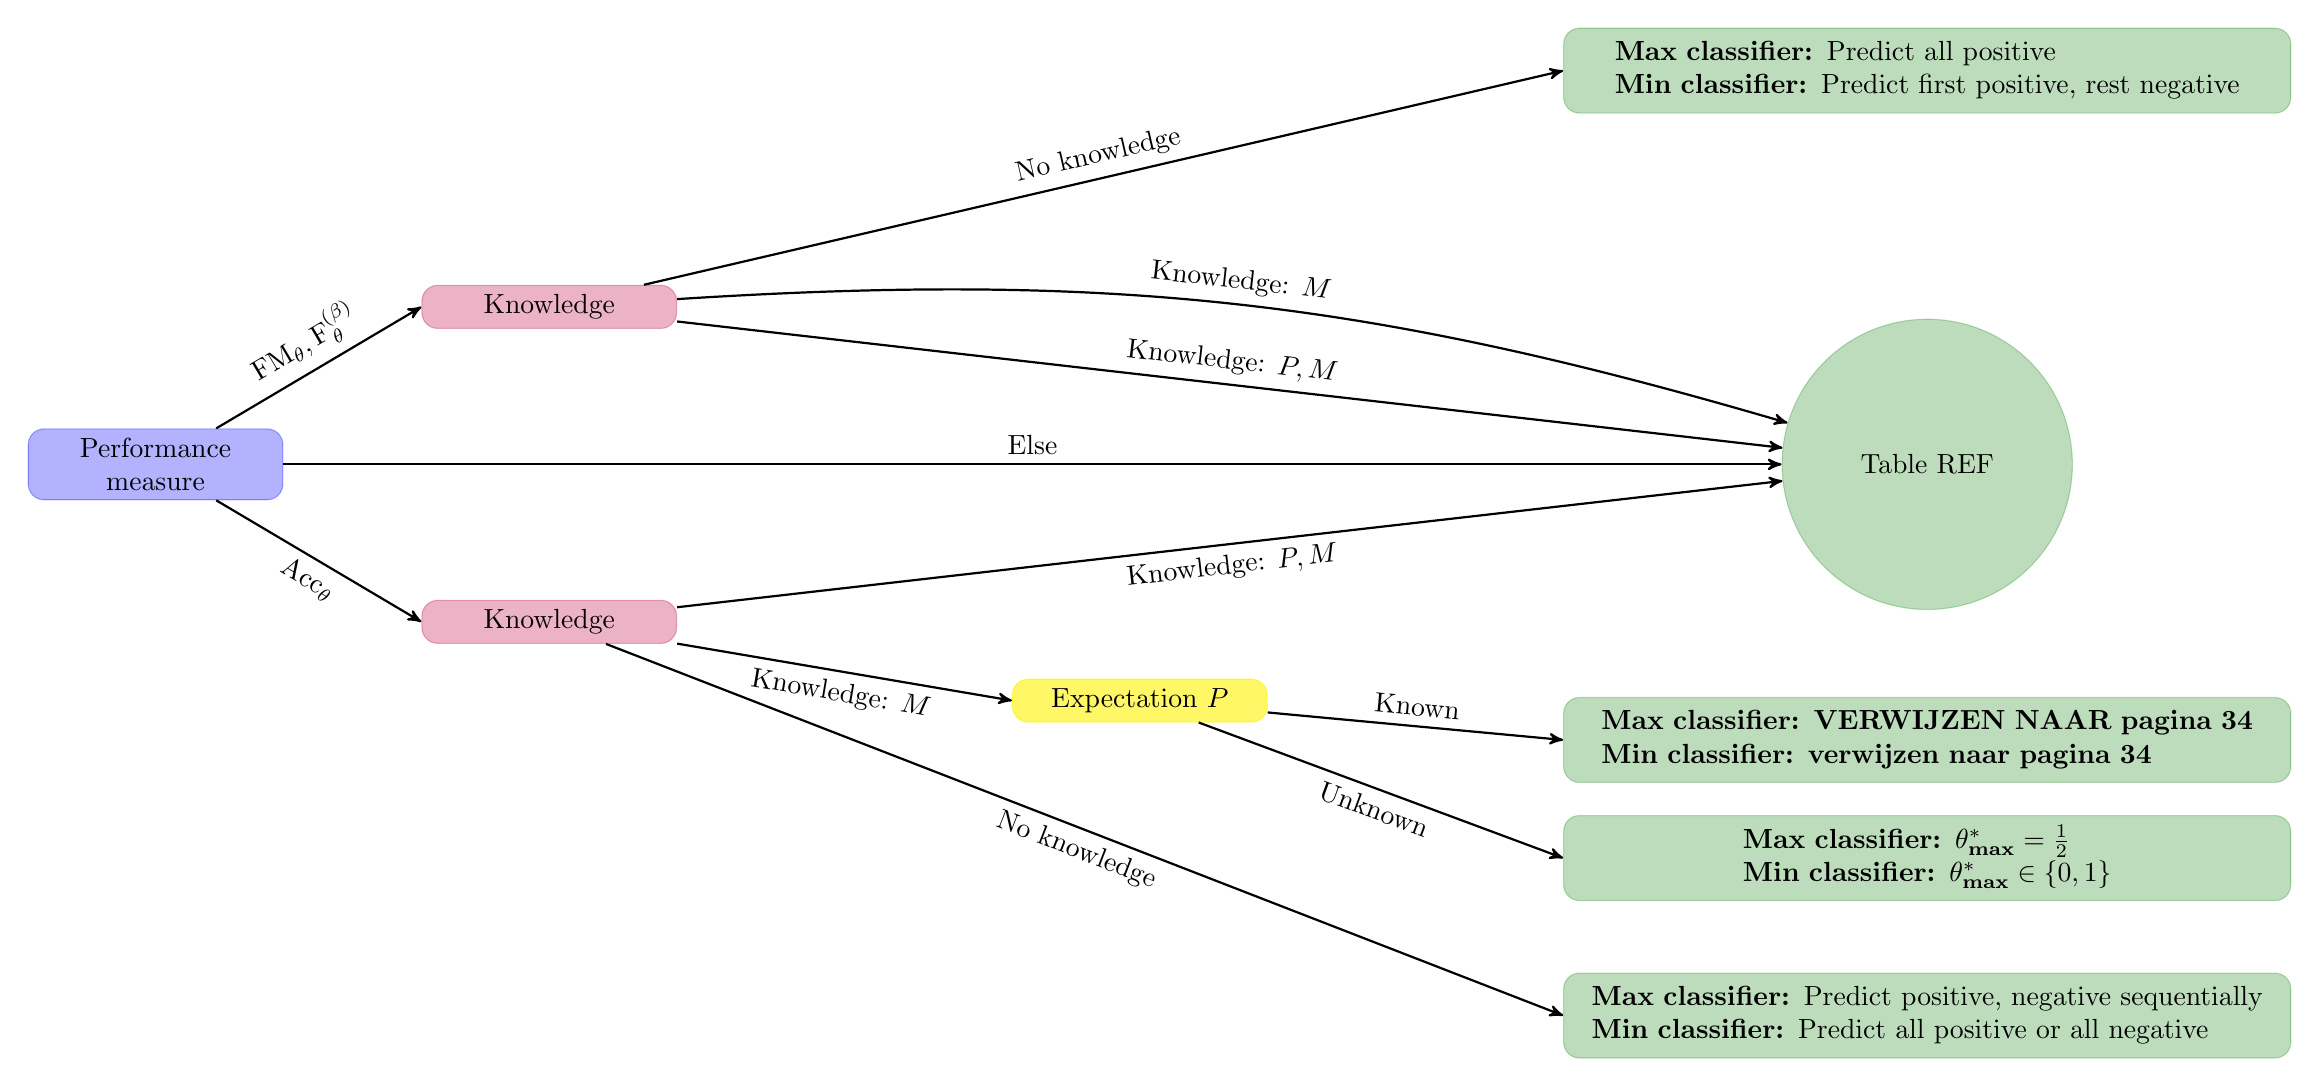
\begin{tikzpicture}
        \def\pointsize{3 cm};
        \def\spacex{5cm};
        \def\spacey{2 cm};
        \node[draw = blue, fill = blue, opacity = 0.3, text opacity = 1, rounded corners = 0.2cm, text width = \pointsize, align = center] (begin) at (0,0){Performance measure};

        \node[draw = purple, fill = purple, opacity = 0.3, text opacity = 1, rounded corners = 0.2cm, text width = \pointsize, align = center] (FMFB) at (\spacex, \spacey){Knowledge};

        \node[draw = purple, fill = purple, opacity = 0.3, text opacity = 1, rounded corners = 0.2cm, text width = \pointsize, align = center] (ACC) at (\spacex,- \spacey){Knowledge};

        \node[draw = ForestGreen, fill = ForestGreen, opacity = 0.3, text opacity = 1, circle, align = center, text width = \pointsize, inner sep = 0.3 cm] (table5) at (4.5 * \spacex, 0){Table REF};

        \draw[->, >=stealth', thick] (begin) -- (FMFB.west) node[above, midway, sloped]{$\text{FM}_{\theta}, \text{F}^{(\beta)}_{\theta}$};

        \draw[->, >=stealth', thick] (begin) -- (ACC.west) node[below, midway, sloped]{$\text{Acc}_{\theta}$};

        \draw[->, >=stealth', thick] (begin) -- (table5) node[above, midway, sloped]{Else};

        \node[draw = ForestGreen, fill = ForestGreen, opacity = 0.3, text opacity = 1, rounded corners = 0.2cm, text width = 3*\pointsize, align = center] (FMFBKNOW) at (4.5 * \spacex, 2.5 * \spacey){
        \begin{tabular}{l}
            \textbf{Max classifier:} Predict all positive \\
            \textbf{Min classifier:} Predict first positive, rest negative
        \end{tabular}
        };





        \node[draw = ForestGreen, fill = ForestGreen, opacity = 0.3, text opacity = 1, rounded corners = 0.2cm, text width = 3 * \pointsize, align = center] (ACCKNOW) at (4.5 * \spacex, -3.5 * \spacey){
            \begin{tabular}{l}
                \textbf{Max classifier:} Predict positive, negative sequentially \\
                \textbf{Min classifier:} Predict all positive or all negative
            \end{tabular}
            };
        \node[draw = yellow, fill = yellow, opacity = 0.6, text opacity = 1, rounded corners = 0.2cm, text width = \pointsize, align = center] (ACCKNOWM)  at (2.5 * \spacex, -1.5 * \spacey){
            Expectation $P$
            };


            \node[draw = ForestGreen, fill = ForestGreen, opacity = 0.3, text opacity = 1, rounded corners = 0.2cm, text width = 3 * \pointsize, align = center] (ACCKNOWM1) at (4.5 * \spacex, -1.75 * \spacey){
                \begin{tabular}{l}
                    \textbf{Max classifier: VERWIJZEN NAAR pagina 34}  \\
                    \textbf{Min classifier: verwijzen naar pagina 34}
                \end{tabular}
                };

                \node[draw = ForestGreen, fill = ForestGreen, opacity = 0.3, text opacity = 1, rounded corners = 0.2cm, text width = 3 * \pointsize, align = center] (ACCKNOWM2) at (4.5 * \spacex, -2.5 * \spacey){
                    \begin{tabular}{l}
                        \textbf{Max classifier: $\theta_{\text{max}}^* = \frac{1}{2}$}  \\
                        \textbf{Min classifier: $\theta_{\text{max}}^* \in \{0, 1\}$}
                    \end{tabular}
                    };


        \draw[->, >=stealth', thick] (FMFB) -- (table5) node[above, midway, sloped]{Knowledge: $P, M$};
        \draw[->, >=stealth', thick] (ACC) -- (table5) node[below, midway, sloped]{Knowledge: $P, M$};
        \draw[->, >=stealth', thick] (FMFB) edge[bend left = 10]node[above, midway, sloped]{Knowledge: $M$} (table5) ;
        \draw[->, >=stealth', thick] (ACC) -- (ACCKNOWM.west) node[below, midway, sloped]{Knowledge: $M$};
        \draw[->, >=stealth', thick] (FMFB) -- (FMFBKNOW.west) node[above, midway, sloped]{No knowledge};
        \draw[->, >=stealth', thick] (ACC) -- (ACCKNOW.west) node[below, midway, sloped]{No knowledge};
        \draw[->, >=stealth', thick] (ACCKNOWM) -- (ACCKNOWM1.west) node[above, midway, sloped]{Known};
        \draw[->, >=stealth', thick] (ACCKNOWM) -- (ACCKNOWM2.west) node[below, midway, sloped]{Unknown};
    \end{tikzpicture}
}

% \resizebox*{0.95\linewidth}{!}{
%     \begin{tikzpicture}
%         \def\helpx{1.2};
%         \def\helpy{2};
%         \draw[fill = blue, opacity = 0.2, rectangle] (0,0) rectangle (11,10);
%         \foreach \x in {5, 4,..., 1} {
%                 \def\midwayx{\helpx + \x - \x / 3}
%                 \draw[opacity = 0.8, fill = white, thick] ({\midwayx + 1}, {\x / 5 + \helpy}) rectangle (\midwayx - 1, {\x/5  + 6 + \helpy});
%                 \ifthenelse{\x=5}{
%                     \foreach \l [count = \i] in {0,1,0,1,1,1} {
%                             \node at (\midwayx, \x / 5 + \helpy + \i  - 1/2){\Huge\l};
%                         }}{}

%                 \ifthenelse{\x=4}{
%                     \foreach \l [count = \i] in {1,1,0,1,1,0} {
%                             \node at (\midwayx, \x / 5 + \helpy + \i  - 1/2){\Huge\l};
%                         }}{}

%                 \ifthenelse{\x=3}{
%                     \foreach \l [count = \i] in {0,0,1,1,1,1} {
%                             \node at (\midwayx, \x / 5 + \helpy + \i  - 1/2){\Huge\l};
%                         }

%                     \def\midwayxx{5.5 + \helpx + 3 - 3 / 3};
%                     \draw[opacity = 0.8, fill = white, thick] ({\midwayxx + 1}, {1 / 5 + \helpy}) rectangle (\midwayxx - 1, {1/5  + 6 + \helpy});
%                     \foreach \l [count = \i] in {0,0,1,1,1,1} {
%                         \node at (\midwayxx, {\helpy + \i - 1/2 + 1/5}){\Huge\l};
%                         }

%                         \coordinate (beginarrow) at ({\helpx + 3 - 3 / 3},{3/5  + 3 + \helpy} );
%                     \coordinate (endarrow) at ({5 + \helpx + 3 - 3 / 3},{3/5  + 3 + \helpy} );
%                     \path[red, ->, >=stealth', very thick] (beginarrow) edge[bend left = 25] node [midway, above, opacity = 0.9, fill = gray!15!white, rounded corners=0.2cm]{Sample uniformly} (endarrow) ;

%                 }{}

%                 \ifthenelse{\x=2}{
%                     \foreach \l [count = \i] in {1,0,1,1,1,0} {
%                             \node at (\midwayx, \x / 5 + \helpy + \i  - 1/2){\Huge\l};
%                         }}{}

%                 \ifthenelse{\x=1}{
%                     \foreach \l [count = \i] in {1,1,0,0,1,1} {
%                             \node at (\midwayx, \x / 5 + \helpy + \i  - 1/2){\Huge\l};
%                         }}{}
%             }
%         \draw [decorate,decoration={brace,amplitude=10pt}]
%         (\helpx + 6 - 5 / 3,2) -- (\helpx - 1 / 3,2) node (allcombinations) [below= 0.5,midway] {\footnotesize
%             All combinations with $\lfloor M\cdot\theta  \rceil$ ones};

%         \node[right = 1.9 of allcombinations] {\footnotesize Predicted labels};

%         \node[anchor = center, text width = 11 cm] at ({11/2}, -1) {\Large \textbf{1. Dutch Draw Classifier:} Predict exactly $\lfloor M\cdot\theta  \rceil$ samples randomly as 1 out of $M$ samples};



%         \tikzset{shift={(15,0)}}
%         \draw[fill = blue, opacity = 0.2, rectangle] (0,0) rectangle (11,10);
%         \def\helpx{2.2};
%         \def\helpy{0.0};
%         \draw[fill = ForestGreen, opacity = 0.3] ({11/ 2}, {\helpy + 10 / 2}) circle (4);
%         \node[fill = white, opacity = 0.9, circle] at (3,4){\footnotesize$\theta = 0.14$};
%         \node[fill = white, opacity = 0.9, circle] at (7,3.2){\footnotesize$\theta = 0.29$};
%         \node[fill = white, opacity = 0.9, circle] at (8.5,6){\footnotesize$\theta = 1.0$};
%         \node[fill = white, opacity = 0.9, circle] at (6,7){\footnotesize$\theta = 0.43$};
%         \node[fill = white, opacity = 0.9, circle] at (4,2.2){\footnotesize$\theta = 0.57$};
%         \node[fill = white, opacity = 0.9, circle] at (2.8,6.5){\footnotesize$\theta = 0.71$};
%         \node[fill = white, opacity = 0.9, circle] at (5,5){\footnotesize$\theta = 0.86$};
%        % \draw [decorate,decoration={brace,amplitude=10pt}]        ({4 + 11/ 2},1) -- ({-4 + 11/2},1) node (circle1) [below= 0.5,midway] {\footnotesize            All Dutch Draw Classifiers};
%        \node[anchor = center, text width = 11 cm] at ({11/2}, -1) {\Large \textbf{2. All Dutch Draw Classifiers:} Family of classifiers for different values of $\theta$};

%         \tikzset{shift={(-15,-15)}}
%         \draw[fill = blue, opacity = 0.2, rectangle] (0,0) rectangle (11,10);
%         \def\helpx{.8};
%         \def\helpy{2};
%         \draw[fill = white, opacity = 0.5, rectangle] (\helpx,\helpy) rectangle (\helpx + 7, \helpy + 6);
%         \draw (\helpx, \helpy) -- (\helpx + 7, \helpy)  node[below, midway, yshift = -4, fill = ForestGreen, opacity = 0.3, rounded corners = 0.2cm, text opacity = 1] {\footnotesize Parameter $\theta$ $\rightarrow$};
%         \draw (\helpx, \helpy) -- (\helpx, \helpy + 6) node[above, midway, rotate = 90, yshift = 4, fill = ForestGreen, opacity = 0.3, rounded corners = 0.2cm, text opacity = 1] {\footnotesize Expectation performance measure $\rightarrow$};

%         \def\ycoord{{2, 0.5, 1,3,4,2,5, 3, 2}}
%         \def\xcoord{{0, 1/2, 3/2, 5/2, 7/2, 9/2, 11/2, 13/2, 7}}
%         \def\i{0};
%         \draw[blue]
%         (\helpx + \xcoord[\i], \helpy + \ycoord[\i]) --
%         (\helpx + \xcoord[\i + 1], \helpy + \ycoord[\i]) --
%         (\helpx + \xcoord[\i + 1], \helpy + \ycoord[\i + 1]);
%         \def\i{1};
%         \draw[blue]
%         (\helpx + \xcoord[\i], \helpy + \ycoord[\i]) --
%         (\helpx + \xcoord[\i + 1], \helpy + \ycoord[\i]) --
%         (\helpx + \xcoord[\i + 1], \helpy + \ycoord[\i + 1]);
%         \def\i{2};
%         \draw[blue]
%         (\helpx + \xcoord[\i], \helpy + \ycoord[\i]) --
%         (\helpx + \xcoord[\i + 1], \helpy + \ycoord[\i]) --
%         (\helpx + \xcoord[\i + 1], \helpy + \ycoord[\i + 1]);
%         \def\i{3};
%         \draw[blue]
%         (\helpx + \xcoord[\i], \helpy + \ycoord[\i]) --
%         (\helpx + \xcoord[\i + 1], \helpy + \ycoord[\i]) --
%         (\helpx + \xcoord[\i + 1], \helpy + \ycoord[\i + 1]);
%         \def\i{4};
%         \draw[blue]
%         (\helpx + \xcoord[\i], \helpy + \ycoord[\i]) --
%         (\helpx + \xcoord[\i + 1], \helpy + \ycoord[\i]) --
%         (\helpx + \xcoord[\i + 1], \helpy + \ycoord[\i + 1]);
%         \def\i{5};
%         \draw[blue]
%         (\helpx + \xcoord[\i], \helpy + \ycoord[\i]) --
%         (\helpx + \xcoord[\i + 1], \helpy + \ycoord[\i]) --
%         (\helpx + \xcoord[\i + 1], \helpy + \ycoord[\i + 1]);
%         \def\i{6};
%         \draw[blue]
%         (\helpx + \xcoord[\i], \helpy + \ycoord[\i]) --
%         (\helpx + \xcoord[\i + 1], \helpy + \ycoord[\i]) --
%         (\helpx + \xcoord[\i + 1], \helpy + \ycoord[\i + 1]);
%         \def\i{7};
%         \draw[blue]
%         (\helpx + \xcoord[\i], \helpy + \ycoord[\i]) --
%         (\helpx + \xcoord[\i + 1], \helpy + \ycoord[\i]);

%         %\draw[scale=1, domain=0:7, smooth, variable=\x, blue] plot ({\helpx + \x}, {\helpy + \x*\x * 6 / 49});
%         \draw[dashed, blue, thick]  (\helpx + 6, \helpy + 6) --  (\helpx + 6, \helpy) node[below]{\footnotesize $\theta^*_{\text{max}}$};
%         \draw[dashed, blue, thick]  (\helpx + 1, \helpy + 6) --  (\helpx + 1, \helpy) node[below]{\footnotesize $\theta^*_{\text{min}}$};

%         \draw[dashed, red, thick] (\helpx, \helpy + 5) --  (\helpx + 7, \helpy + 5) node [right = 0.2] (maximize) {\footnotesize Maximizing baseline};
%         \draw[dashed, red, thick] (\helpx, \helpy + 0.5) --  (\helpx + 7, \helpy + 0.5) node [right = 0.2] (minimize) {\footnotesize Minimizing baseline};


%         \node[anchor = center, text width = 11 cm] at ({11/2}, -1) {\Large \textbf{3. Optimal Dutch Draw Classifier:} Determine the optimal Dutch Draw Classifier using the expectation of the performance measure};


%         \tikzset{shift={(15, 0)}}
%         \draw[fill = blue, opacity = 0.2, rectangle] (0,0) rectangle (11,10);
%         \def\helpx{2};
%         \def\helpy{3};
%         \node[anchor = center, fill = white, opacity = 0.9, inner sep = 1 cm] (dutchdrawbaseline) at ({11/2}, {\helpy + 10 / 2}) {\Huge Dutch Draw Baseline};
%         \path[red, <-, >=stealth', very thick] (minimize) edge[bend right = 25] ({11/2}, {\helpy + 9 / 2});
%         \path[red, <-, >=stealth', very thick] (maximize) edge[bend right = 45] ({11/2}, {\helpy + 9 / 2});


%         \node[anchor = center, text width = 11 cm] at ({11/2}, -1) {\Large \textbf{4. Dutch Draw Baseline:} Optimal performance of a Dutch Draw Classifier};

%         \def\spacey{0.9};
%         \node[opacity = 0.3, text opacity = 1, fill =ForestGreen, rounded corners=0.2cm, text width = 10cm, align = center] at({11/2}, 6) {\large \ding{51}  applicable in any binary classification problem};
%         \node[opacity = 0.3, text opacity = 1, fill =ForestGreen, rounded corners=0.2cm, text width = 10cm, align = center] at({11/2}, {6 - \spacey}) {\large \ding{51}  theoretical derivations};
%         \node[opacity = 0.3, text opacity = 1, fill =ForestGreen, rounded corners=0.2cm, text width = 10cm, align = center] at({11/2}, {6 - 2 * \spacey}) {\large \ding{51}  reproducible};
%         \node[opacity = 0.3, text opacity = 1, fill =ForestGreen, rounded corners=0.2cm, text width = 10cm, align = center] at({11/2}, {6 - 3 *\spacey}) {\large \ding{51}  simple};
%         \node[opacity = 0.3, text opacity = 1, fill =ForestGreen, rounded corners=0.2cm, text width = 10cm, align = center] at({11/2}, {6 - 4 *\spacey}) {\large \ding{51}  parameter-free};
%         \node[opacity = 0.3, text opacity = 1, fill =ForestGreen, rounded corners=0.2cm, text width = 10cm, align = center] at({11/2}, {6 - 5 *\spacey}) {\large \ding{51}  more informative than any dummy classifier};
%         \node[opacity = 0.3, text opacity = 1, fill =ForestGreen, rounded corners=0.2cm, text width = 10cm, align = center] at({11/2}, {6 - 6 *\spacey}) {\large \ding{51}  explainable minimal requirement for new model};
%     \end{tikzpicture}
% }

% \section*{Proof that Dutch Sample is superior}

% \Joris{Misschien nog extra restricties op de measure $\mu$ leggen, bijvoorbeeld dat deze niet positie-afhankelijk is}


% Let $\mathbf{X} := [\mathbf{x}_1 \dots \mathbf{x}_M]^T$ be the set of all explanatory feature values corresponding to the samples $1,\dots, M$. Let $S(X)$ be the set of all permutations over the samples.


% Let $P$ denote the number of positives and $N$ the number of negatives. Note that $P + N = M$.

% We are interested in the following set of classifiers, that only use the information: $P$, $N$ and $M$.

% \begin{definition}
%     The set of possible classifiers that only use the information $P$, $N$ and $M$ is $C$ with \begin{align*}
%         C &= \{W: \mathbb{R}^{M\times K} \oplus \mathbbm{N} \oplus \mathbbm{N} \oplus \mathbbm{N} \to \{0,1\}^M , \mathbf{X} \mapsto f_W(P, N, M) \}
%     \end{align*}
% \end{definition}

% \begin{align*}
%     f_W(P,N,3) &= \left \{ \begin{array}{ll}
%         (1,0,0) & \text{met kans } \frac{P}{M}\\
%         (0,0,1) & \text{met kans } \frac{N}{M}
%     \end{array} \right.
% \end{align*}



% \begin{definition}
%     The set of possible classifiers that only use the information $P$, $N$ and $M$ is $C$ with \begin{align*}
%         C &= \{W: (P,N,M) \to \{0,1\}^M  \}
%     \end{align*}
% \end{definition}


% \newpage
% Let $W\in C$ and note that $W(\mathbf{X})$ can be stochastic.

% Let $W$ be a classifier that uses no knowledge. Let $\bm{X}$ be the set of samples and let $S(\bm{X})$ be the set of all permutations of these samples. Note that $W$ can be stochastic, thus given an instance $x\in S(\bm{X})$ the result $W(x)$ is stochastic.

% This is annoying, thus we will decompose $W$ into unique deterministic classifiers $(w_1, \dots, w_{2^{|\bm{X}|}})$ and define probability $p_i(x) = \PP(W(x) = w_i(x))$.

% However, $W$ uses no knowledge of $x$, \Joris{No positional knowledge!}thus it must hold that $p_i(x)=: p_i$ is constant for all $x$.

% Note that $W(x) = W(\cdot)$ for all $x$ and $w_i(x) = w_i(\cdot)$


% Let $\mu$ denote an evaluation measure. Then \begin{align*}
%     \EE[\mu(W(x))] &=\sum_i p_i(x) \cdot \mu (w_i(x)) \\
%     &=  \sum_i p_i \cdot \mu (w_i(x))
% \end{align*}

% We assume that the test set is randomly shuffled, thus if a classifier is superior than the dutch sample, we have to take into account that we take the expectation over all possible shuffles of the test set. Let $\sigma_{\THO}$ be the optimal shuffle approach. If $W$ is better than the shuffle, it must hold that \begin{align*}
% &\EE_{x \in S(\bm{X})}\left [ \EE[\mu(W(x))] \right ] > \EE_{x \in S(\bm{X})}\left [ \EE[\mu(\sigma_{\THO}(x))] \right ]\\
% & \leadsto \EE_{x \in S(\bm{X})}\left [ \sum_i p_i \cdot \mu (w_i(x)) \right ]> \EE_{x \in S(\bm{X})}\left [ \EE[\mu(\sigma_{\THO}(x))] \right ]\\
% & \leadsto  \sum_i p_i \cdot \EE_{x \in S(\bm{X})}\left [\mu (w_i(x)) \right ]> \EE_{x \in S(\bm{X})}\left [ \EE[\mu(\sigma_{\THO}(x))] \right ]\\
% \end{align*}
% Furthermore, we have:
% \begin{align*}
%     \sum_i p_i \cdot \EE_{x \in S(\bm{X})}\left [\mu (w_i(x)) \right ] \leq \max_{i} \{\EE_{x \in S(\bm{X})}\left [\mu (w_i(x)) \right ] \}
% \end{align*}
% as $\sum_i p_i = 1$ and $p_i \leq 1$ for all $i$.

% Let $i_{max} \in \argmax_i \{ \EE_{x \in S(\bm{X})}\left [\mu (w_i(x)) \right ] \}$.

% Note that due to the expectation over all possible shuffles of the test set in the expectation $\EE_{x \in S(\bm{X})}\left [\cdot  \right ]$, the expected performance of classifier $w_i$ is the same as any permutation $\pi$ of this classifier, so:
% \begin{align*}
%     \EE_{x \in S(\bm{X})}\left [\mu (w_i(x)) \right ] &= \EE_{x \in S(\bm{X})}\left [\mu (\pi(w_i(x))) \right ].
% \end{align*}

% This entails that only the number of samples that are positively labeled is of importance. If another classifier $w_j$ classifies the same number of positives, it must hold that
% \begin{align*}
%     \EE_{x \in S(\bm{X})}\left [\mu (w_i(x)) \right ] &= \EE_{x \in S(\bm{X})}\left [\mu (w_j(x)) \right ],
% \end{align*}
% as we can find a permutation such that $\pi(w_j(\cdot)) = w_i(\cdot)$.

% Thus, it must hold that $j \in  \argmax_i \{ \EE_{x \in S(\bm{X})}\left [\mu (w_i(x)) \right ] \}$ if $w_j$ predicts as many positives as $w_{i_{max}}$. Denote the number of positives by $\hat{P}_i$ for classifier $w_i$.

% Observe that if we take the Dutch Sample with $\theta = \frac{\hat{P}_{i_{max}}}{M}$, we predict exactly $\hat{P}_{i_{max}}$ positives. Thus  \begin{align*}
%     \EE_{x \in S(\bm{X})}\left [\mu (w_{i_{max}}(x)) \right ] = \EE_{x \in S(\bm{X})}\left [\mu (\sigma_{\frac{\hat{P}_{i_{max}}}{M}}(x)) \right ]
% \end{align*}

% So \begin{align*}
%     \EE_{x \in S(\bm{X})}\left [\mu (\sigma_{\frac{\hat{P}_{i_{max}}}{M}}(x)) \right ] &= \EE_{x \in S(\bm{X})}\left [\mu (w_{i_{max}}(x)) \right ] \\
%     & = \max_{i} \{\EE_{x \in S(\bm{X})}\left [\mu (w_i(x)) \right ] \} \\
%     & \geq \sum_i p_i \cdot \EE_{x \in S(\bm{X})}\left [\mu (w_i(x)) \right ]\\
%     & >\EE_{x \in S(\bm{X})}\left [ \mu(\sigma_{\THO}(x)) \right ]
% \end{align*}

% This leads to a contradiction, as there is apparently a more optimal $\theta$.



% \definecolor{ballblue}{rgb}{0.13, 0.67, 0.8}
% \definecolor{persianpink}{rgb}{0.97, 0.5, 0.75}

% \definecolor{color1}{rgb}{0.31, 0.78, 0.47}
% \definecolor{color2}{rgb}{0.0, 0.47, 0.44}
% \definecolor{color3}{rgb}{0.11, 0.35, 0.02}

% \newtcolorbox{mybox}[2][]{
%     box align = center,
% halign = center,
% width = 6 cm,
% colback=red!5!white,
% colframe=red!75!black,
% colbacktitle=red!85!black,enhanced,
% attach boxed title to top center={yshift=-2mm},
% title=#2,#1}


% \resizebox*{\linewidth}{!}{
% \begin{tikzpicture}
% \node[draw = black, fill = gray!15, rounded corners, inner sep = 13pt, anchor = center] (first) at (0,0){All Dutch Draw classifiers};

% %%%%%%%%%%%%%%%%%%%%%%%%%%%%%%%%%%%%%%
% \node[above right = 2cm of first] (firstbranchopt) {   \begin{mybox}[colback=gray!15, colframe = color1, colbacktitle = color1]{{Knowledge: $P, M$}}
%     Optimal Dutch Draw classifier
%     \end{mybox}};
% \node[right = 2cm of firstbranchopt] (firstbranchbase){   \begin{mybox}[colback=gray!15, colframe = color1, colbacktitle = color1]{{Knowledge: $P, M$}}
%     Dutch Draw baseline
%     \end{mybox}};

% \draw[->, ultra thick, shorten >=3pt, shorten <=3pt, ballblue] (first) |- node [above, near end]{(1)} ($(firstbranchopt) + (-3 cm, -0.2 cm)$);

% \draw[->, ultra thick, shorten >=3pt, shorten <=3pt, persianpink] ($(firstbranchopt) + (3 cm, -0.2 cm)$) -- node [above, midway]{(2)} ($(firstbranchbase) + (-3 cm, -0.2 cm)$);

% %%%%%%%%%%%%%%%%%%%%%%%%%%%%%%%%%%%%%%%%

% \coordinate[below right = 2cm of first] (help1);


% \node (thirdbranchopt) at ([yshift = -5.25 cm]firstbranchopt) {
%     \begin{mybox}[colback=gray!15, colframe = color3, colbacktitle = color3]{{No knowledge}}
%         Optimal Dutch Draw classifier
%         \end{mybox}
% };

% \node[right = 2cm of thirdbranchopt] (thirdbranchbase){    \begin{mybox}[colback=gray!15, colframe = color3, colbacktitle = color3]{{No knowledge}}
%   Dutch Draw baseline
%     \end{mybox}};

% \draw[->, ultra thick, shorten >=3pt, shorten <=3pt, ballblue] (first) |- node [above, near end]{(1)} ($(thirdbranchopt) + (-3 cm, -0.2 cm)$);

% \draw[->, ultra thick, shorten >=3pt, shorten <=3pt, persianpink] ($(thirdbranchopt) + (3 cm, -0.2 cm)$) -- node [above, midway]{(2)} ($(thirdbranchbase) + (-3 cm, -0.2 cm)$);


% %%%%%%%%%%%%%%%%%%%%%%%%%%%%%%%%%%%%%%%%%%%%%%%%%%%%%%%%%

% \coordinate (midway1) at ($(firstbranchopt)!0.5!(thirdbranchopt)$);

% \node (secondbranchopt) at ($(midway1) + (0, 0.0cm)$) {
%     \begin{mybox}[colback=gray!15, colframe = color2, colbacktitle = color2]{{Knowledge: $M$}}
%         Optimal Dutch Draw classifier
%         \end{mybox}
% };

% \node[right = 2cm of secondbranchopt] (secondbranchbase){    \begin{mybox}[colback=gray!15, colframe = color2, colbacktitle = color2]{{Knowledge: $M$}}
%   Dutch Draw baseline
%     \end{mybox}};

% \draw[->, ultra thick, shorten >=3pt, shorten <=3pt, ballblue] (first) -- node [above, midway]{(1)} ($(secondbranchopt) + (-3 cm, -0.2 cm)$);

% \draw[->, ultra thick, shorten >=3pt, shorten <=3pt, persianpink] ($(secondbranchopt) + (3 cm, -0.2 cm)$) -- node [above, midway]{(2)} ($(secondbranchbase) + (-3 cm, -0.2 cm)$);


% %%%%%%%%%%%%%%%%%%%%%%%%%%%%%%%%%%%%%%%%%%%%%%%%%%%%%%%%%




% \node (knooppunt1) at (-2.5 cm, -5 cm){};
% \node[right= 2 cm of knooppunt1] (uitleg1){: For a given measure determine the optimal classifier with/without knowledge of $P$, $M$.};
% \draw[->, ultra thick, shorten >=3pt, shorten <=3pt, ballblue] (knooppunt1) -- node [above, midway]{(1)} ++(2 cm,  0);

% \node (knooppunt2) at (-2.5 cm, -6 cm){};
% \node[right= 2 cm of knooppunt2] (uitleg2){: Determine the performance of the optimal Dutch Draw classifier with/without knowledge of $P$, $M$.};
% \draw[->, ultra thick, shorten >=3pt, shorten <=3pt, persianpink] (knooppunt2) -- node [above, midway]{(2)} ++(2 cm,  0);


% \node at (8 cm , 6 cm) {\Large \bfseries The Dutch Draw};


% \end{tikzpicture}
% }









\end{document}
